\section{Introduction}
Variable resolution grids have been used in regional atmospheric models for several decades
\citep{fox1997finite}. The most common downscaling approach was the nested grid, in which
a fixed-size refined grid is embedded within the coarse grid at a set location. It was implemented in several
limited area models (LAM) for local weather forecasting
and regional climate simulations (e.g. \cite{Phillips1979nested}, \cite{pielke1992comprehensive}, \cite{grell1994description},
and \cite{caya1999semi}). Many of these models are regularly used today.
For example, one of the most frequently used LAMs with embedded nested grids is the
Weather Research and Forecasting Model (WRF, \cite{Skamarock:2008db}).

An alternative approach to downscaling designed for global 
models is the stretched grid that was developed
around the same time \citep{Schmidt:1977qo, staniforth1978variable}. 
In these models, an originally
uniform mesh is smoothly distorted such that more grid elements are concentrated
over a localized region, providing higher resolution in that area and leaving 
fewer grid elements, and thus coarser resolution, 
in the remaining area. Stretched grids require few modifications to the
numerical schemes and computational grids to implement in general circulation models (GCMs). 
Thus they were an attractive technique to 
implemented in variable resolution modeling because GCMs avoid many drawbacks 
associated with LAMs such as lateral boundary conditions and their inability
to capture upscaling effects. Several stretched grid models developed
at that time include \cite{paegle1989variable}, \cite{deque1995high},
\cite{yessad1996introduction}, \cite{fox1997finite}, and \cite{cote1998operational}).

Early
GCMs using nested grids were developed by \cite{Ruge:1995cy} and \cite{dudhia2002global}.
Nested grids within GCMs involve continuous two-way 
communication between resolutions and require more challenging numerical
schemes and computational grids.
This made them initially less attractive in comparison to stretched grids. 
A second form of nesting involves a single grid spanning multiple resolutions, where refined
grid cells physically replace the coarse cells in the region of interests.
An early example of this technique was implemented by \cite{Fournier:2004cf}.

With the advancement of large-scale parallel computing systems,
variable resolution GCMs are
a growing fixture in atmospheric and climate modeling. Variable resolution has been 
incorporated into several operational GCMs across major modeling centers 
\citep{skamarock2012multiscale,Harris:2013nt,zarzycki2014aquaplanet}.
This combination has proven to be effective for assessing
tropical cyclones \citep{zarzycki2014multidecadal, zarzycki2015tropical, huang2017influences}, 
large-scale weather systems \citep{rauscher2014impact}, atmospheric rivers \citep{hagos2015resolution},
 and regional climate \citep{medvigy2013simulated, huang:16, gettelman2017regional, rhoades2018projecting}.
Specifically, variable resolution can bridge the difference in 
scale between global and regional climate modeling by overcoming
many of the known issues with conventional downscaling methods of LAMs or high resolution GCMs.
They provide high-resolution in a desired location while eliminating the need for forced lateral boundary conditions, 
capture small-to-large scale teleconnections, and demand fewer computational
resources compared to standard uniform high-resolution GCMs.

The variable resolution models discussed thus far implement static grid refinement.
The refined grid's location is determined \emph{a priori} and remains fixed for
the entirety of the simulation. Dynamic grid refinement, such as adaptive mesh refinement (AMR),
is a more flexible variable resolution modeling technique. Adaptive grids track features of interest
and refine the grid locally in advance of any important physical features or processes requiring
additional resolution. When the additional resolution is no longer needed, that same region of
the grid is coarsened.
While dynamic refinement is frequently implemented in other areas of computational 
hydrodynamics such as aerospace and heliophysics, it has not been widely adapted
for atmospheric and climate modeling. Since dynamically adaptive grids were first
applied to atmospheric flows by \cite{skamarock1989adaptive},
\cite{skamarock1993adaptive} and \cite{Dietachmayer:1992sj}, adaptive model
work has been limited to algorithm development, simplified models, and idealized simulations.
Dynamically adaptive shallow water models on the sphere have been discussed in
\cite{giraldo2000lagrange}, \cite{behrens2005amatos}, \cite{lauter2007parallel}, 
\cite{st2007comparison}, \cite{kubatko2009dynamic}, and \cite{Chen:2011kk}.
More recent model designs have been presented in \cite{mccorquodale2015adaptive},
\cite{tumolo2015semi}, \cite{aechtner2015conservative}, and \cite{weller2016mesh}.
Several applications of AMR and dynamic refinement in the shallow water system 
include tsunami propagation in \cite{blaise2012dynamic}, Fujiwhara interactions in
\cite{bauer2014simulation}, and tropical cyclone eye-wall evolution in
\cite{hendricks2016evaluation}. \cite{ferguson2016analyzing} provides
more detailed overview of these models and their dynamic refinement techniques.
 Though some LAM models like 
WRF \citep{shepherd2017sensitivity} have primitive 
moving nested grids, these cannot be considered true AMR models. 
The nests in these models are often fixed in size and grid elements cannot 
be added or removed. The only full 
3D atmospheric model with dynamic refinement known is the OMEGA
model by \cite{bacon2000dynamically}. This adaptive non-hydrostatic limited-area model
implemented on rotated Cartesian coordinates has been used as a regional hurricane
forecasting system in \cite{gopalakrishnan2002operational}.

This chapter explores the use of mapped-multiblock AMR techniques for three-dimensional 
atmospheric flows. We use the nonhydrostatic finite-volume Chombo
AMR model on the cubed-sphere extended to the full 3D atmospheric equations from the 
2D shallow water model of \cite{mccorquodale2015adaptive}. We wish to
characterize the ability of this model and its multiblock refinement
to simulate atmospheric flow in the global 3D system. To this end, we 
implement the \cite{lin2017colliding} modon test case in the dynamical core (dycore) without any
forcing or subgrid physical parameterization. We run convergence tests and 
demonstrate the use of AMR with simple tagging criteria to observe how
effectively AMR resolves and tracks the modons. We also implement a second
test case, the idealized tropical cyclone from \cite{reed2011vortex}, in which a single,
idealized initial weak vortex evolves into a tropical cyclone. This test requires
the simplified physics scheme from \cite{reed2012idealized} consisting of parameterizations for large-scale condensation,
boundary layer diffusion, and surface fluxes for moisture, sensible heat, and
momentum. With the idealized vortex, we investigate the AMR's ability to track and resolve
the strengthening cyclone using various refinement criteria and thresholds to trigger 
refinement. The results presented are an preliminary assessment of
the AMR capabilities of the 3D models. This model is still undergoing development and
we are currently discovering, evaluating, and resolving instabilities. Several of these issues are noted in
following sections.

This chapter proceeds as follows. Section \ref{sec:experimental} contains a brief description of the 
the nonhydrostatic 3D finite-volume model on the cubed-sphere.
In section \ref{sec:modon}, we present the results of the colliding modon test,
including convergence tests.  The results of
the idealized tropical cyclone test and the comparisons of
various AMR refinement criteria are discussed in section \ref{sec:tctest}. In Section
\ref{sec:conclusion3} we summarize our conclusions and comment on the direction of future
research.

\section{Experimental design}
\label{sec:experimental}

The non-hydrostatic finite-volume Chombo AMR model
is a global 3D model built upon the shallow water version presented in \cite{mccorquodale2015adaptive}.
The dycore utilizes the full-non-hydrostatic moist fluid equations in a shallow-atmosphere
approximation on a cubed-sphere grid.

\subsection{Cubed-Sphere Grid}
The cubed-sphere grid, first developed by \cite{sadourny1972conservative}, consists of a cube with six Cartesian panels inflated out to form a spherical shell.
The grid avoids this pole-problem of traditional latitude-longitude grids by replacing the two strong singularities at the poles with eight weaker singularities at
the corner points of the originally cube. The cubed-sphere grid also provides a near uniform tiling of the sphere as compared to
large changes in grid spacing on the latitude-longitude mesh. 
There are multiple ways to map the grids of each panel to the sphere (see \cite{putman2007finite} for a review
of several cubed sphere grids).  The Chombo-AMR model uses gnomonic equiangular cubed-sphere grid, where the
gridlines on each panel have equally spaced central angles relative to the center of the sphere. This projection
yields a quasi-uniform spherical grid. The grid does not have perfectly uniform tile sizes, but as resolution increases
the ratio between the largest and smallest grid cells converges to $\sqrt{2}$, the smallest ratio of cubed-sphere
grids. Figure \ref{fig:cubedsphere2dmaps} depicts the equiangular cubed-sphere grid.

\begin{figure}[htp]
\centerline{
\includegraphics[width=4in]{Chap3/cubedsphere12456.pdf}                                                                                        
}
\caption{
A cubed-sphere grid, shown with labels on panels.                                                                                                             
Panels 1 -- 4 all straddle the equator
($z = 0$) of the unit sphere.
Panel 5 is centered on the north pole ($z = +1$),
panel 6 on the south pole ($z = -1$).
On the cubed-sphere grid shown here,
$N_{\rm c} = 16$ (each panel contains $16 \times 16$ grid cells).
}
\label{fig:cubedsphere2dmaps}
\end{figure}

The physical domain of the model 
is a spherical shell $r \in [R_i,R_f]$ with a thickness of $H = (R_f - R_i)$,
where $R_i$ and $R_f$ are the radii of the model 
bottom and top respectively, and the assumption 
that $H \ll R_i, R_f$. This shallow 
atmosphere assumption allows us to neglect $r$ metric
dependencies (e.g. no area increase with altitude).
The physical domain is mapped from the cubed-sphere grid.

The equiangular coordinates system for the 
cubed-sphere grid is given as $(\alpha, \beta, \xi, n_p)$, defined
on six panels $n_p \in [1,2,\dots, 6]$, with central angles $\alpha, \beta \in [-\frac{\pi}{4},\frac{\pi}{4}]$ and 
vertical coordinate $\xi \in [0,1]$. By convention, panels 1-4 are along the 
equator and panels 5 and 6 are centered on the north and south poles,
respectively, as seen in Fig. \ref{fig:cubedsphere2dmaps}. 
Each panel is discretized into an $N_c \times N_c$ grid of quadrilaterals.
The edges of each grid cell are non-orthogonal 
segments of the great circle in either the $\alpha$ or $\beta$ direction. 
This property makes the computational grid sizes constant so that
$d\alpha = d\beta = \frac{\pi}{2N_c}$. 
The discrete horizontal resolution of the cubed-sphere grid is represented as  $c\{N_c\}$.
A list of the horizontal properties of the equiangular cubed-sphere grid, including the
approximate grid spacings, and comparable resolutions for other coordinate systems, is given in
Table~\ref{tb:grids} for several resolutions.

The vertical direction is discretized into $N_v$ layers 
with non-constant thickness but constant thickness in the 
computational domain so that for each level $\Delta \xi = 1/N_v$.
The mapping $r(\xi)$ between the physical and computational 
domains is such that
$r(\xi=0) = R_a$ and $r(\xi=1) = R_a + H$ where $R_a$ is the radius of 
the spherical shell and $H$ is the height of the model top. 
The height-based vertical mapping is set by a user-created 
array consisting of the coordinate positions for the vertical level interfaces in physical space.
For non-uniformly spaced vertical maps, the final positioning of the 
level interface points are smoothed via a cubic spline.


\subsection{Fluid equations in cubed-sphere coordinates}
The dycore utilizes the following state variables
\begin{equation}
\label{eq:imexsplit}
\bS
  = 
\begin{bmatrix}
  \avg{J \rho \ua} \\
  \avg{J \rho \ub} \\
  [w]_f \\
  [p]_c \\
  \avg{J \rho} \\
  \avg{J \rhoth} \\
  \avg{J \rhoqv} 
\end{bmatrix}.
\end{equation}
Angled brackets $\avg{}$ indicate a cell averaged variable for the density $\rho$, the horizontal 
momentum density variables $\rho \ua$ and $\rho \ub$ in the $\alpha$ and
 $\beta$ directions on the cubed-sphere, respectively.
The virtual potential temperature is $\theta_v$ and the 
specific humidity $q_v$ which will serves as a placeholder for other physics tracers. 
Vertical velocity $w$ is face-centered variable indicated by $[]_f$ and 
pressure $p$ is a cell-centered variable, indicated by $[]_c$.
$J$ is the metric Jacobian.
The relationship
between the physical vertical velocity $w$ and the computational vertical velocity $\uxi$ 
is given by
\begin{equation}
w = r_{\xi}\uxi.
\end{equation}
The relationship between the derivates in the computational 
vertical coordinate $\xi$ and physical vertical coordinate $r$
is
\begin{equation}
  \partial_r = r_{\xi}^{-1} \partial_{\xi}.
\end{equation}
In both equations, $r_{\xi}$ is the vertical coordinate transform term for converting
between physical and computational spaces.
The virtual potential temperature is defined as
\begin{equation}
\theta_v = (1-0.61q_v)T\left(\frac{p_0}{p}\right)^\kappa,
\end{equation}
where $T$ denotes the temperature, $p_0=10^5$ Pa is the reference pressure and $\kappa = R_d /c_{pd}$.
Here $R_d$ is the ideal gas constant and $c_{pd}$ is the specific heat at constant 
pressure, both in the case of dry air.

With these variables the equations of motion in conservation form on the cubed sphere grid are:
\begin{align}
\frac{\partial J \rho \ua}{\partial t} &=  - \sum_{i=\alpha, \beta} \partial_i (J \rho \ua u^i + JG^{\alpha i} p )
    - \dxi (J \rho \ua \uxi + JG^{\alpha \xi} p)  + J \Psi_C^\alpha + J \Psi_M^\alpha\\
\frac{\partial J \rho \ub}{\partial t} &=  - \sum_{i=\alpha, \beta} \partial_i (J \rho \ub u^i + JG^{\beta i} p )
    - \dxi (J \rho \ub \uxi + JG^{\beta \xi} p)
    + J \Psi_C^\beta + J \Psi_M^\beta \\
\frac{ \partial w}{\partial t} &=   - \sum_{i=\alpha, \beta} u^i \partial_i w - \uxi \, \dxi w - \frac{1}{\rho} \dr p - g \\
\frac{\partial p}{\partial t} &=   - \sum_{i=\alpha, \beta} \left( \gamma p \frac{1}{J} \partial_i (J u^i) 
    + u^i \partial_i p \right) - \uxi \dxi p  - \gamma p \, \dr w  + \eta \left(P(\rhoth) -p \right) \label{eq:eompress}\\
\frac{ \partial J \rho}{\partial t} &=  - \sum_{i=\alpha, \beta} \partial_i (J \rho u^i) - \dxi ( J \rho \uxi ) \\
\frac{ \partial J \rhoth}{\partial t} &=  - \sum_{i=\alpha, \beta} \partial_i (J \rhoth u^i) - \dxi ( J \rhoth \uxi ) \\
\frac{ \partial J \rhoqv}{\partial t} &=  - \sum_{i=\alpha, \beta} \partial_i (J \rhoqv u^i) - \dxi ( J \rhoqv \uxi )
\end{align}
where $G^{ij}$ represent the contravariant cubed-sphere metric term, $g$ is the acceleration
due to gravity, and $\gamma = 1 / (1 - \kappa)$. $\Psi_C$ and $\Psi_M$ represent source terms
from the Coriolis force and metric terms due to the cubed-sphere geometry, respectively. 
These source terms and coordinate transforms that arise from using cubed-sphere mapping may be found in
Appendices A and B of \cite{ullrich2012mcore}.
Currently no topography is implemented. 
Finally the moist equation of state for the equations of motion is
\begin{equation}
\label{eq:eos}
P = p_0\left(\frac{R_d\rhoth}{p_0}\right)^\gamma.
\end{equation}

Equation \ref{eq:eompress} includes a volume discrepancy term: $\eta \left(P(\rhoth) -p \right)$ 
with relaxation parameter $\eta = 0.5 $ to prevent the 
prognostic pressure $p$ from drifting from the equation of state pressure $P$. 
The volume discrepancy approach is used in gas dynamics 
modeling to couple non-linear explicit flow solvers and stiff 
reactions and to maintain conservation in potential 
temperature density \citep{day2000numerical}. Because the equations
of motion are closed with the equation of state Eq. \ref{eq:eos}, this leads to a non-linearity in
$\theta_v$ which leads to pressure values drifting apart. Note that the redundant pressure equation
makes it convenient to treat acoustic waves implicitly. 
The volume discrepancy term relaxes the prognostic pressure to the equation of state pressure.

\subsection{Numerical Methods}
The non-hydrostatic equations are spatially discretized with a finite-volume scheme 
that was implemented by \cite{mccorquodale2015adaptive} for the shallow water equations.
The 3D scheme computes the horizontal fluxes with fourth-order accuracy, but is only accurate
to second-order in the vertical.  To perform the finite volume calculations on panel edges, the 
mapped-multiblock approach creates three layers of ghost cells 
and remaps the values from neighboring cells to these ghost cells. 
 In addition, a sixth-order diffusive operator which maintains the fourth-order 
 accuracy of the scheme is applied to the horizontal fluxes. 
There is no dissipation in the vertical. The numerical scheme is 
mass-conserving to machine precision and energy-conserving up to the
temporal truncation order, when used without limiters or explicit
dissipation. Since topography is not yet mplemented in the dycore, 
simple height-based vertical coordinates are used.

Time integration is conducted by an implicit-explicit second-order, three stage 
ARS232 scheme by \cite{ascher1997implicit}. Given the 
large aspect ratio in the vertical direction, vertical acoustic waves, which are supported by
the shallow atmosphere equations of motion, would severely limit the global time step.
Thus, the terms responsible for vertical acoustic waves in the $w$ and $p$ equations are separated out to
be treated implicitly. All the horizontal terms and the remaining advection terms for the vertical
variables are evaluated explicitly.

The mapped-multiblock AMR techniques developed from the Chombo library \citep{Adams:2015gd} 
and used for the shallow water model in \cite{mccorquodale2015adaptive} and \cite{ferguson2016analyzing}
are implemented in the full 3D dycore.
AMR calculations are performed on a hierarchy of nested meshes, called
levels, which have a defined refinement ratio between them. 
The finer levels are overlaid on top of the coarser levels.  Information on these finer
level is initialized via interpolations from the coarser level and ghost cells 
are used to calculated the fluxes at patch boundaries. Information from the finer level
is averaged down to update values on the coarser level.
These levels are sub-cycled in time to maintain a constant Courant
number across all levels. A detailed overview of the AMR level strucutre and
sub-cycling time integration is provided in Chapter \ref{chap:basicsw}.
Refinement is only done in the horizontal direction, vertical refinement is not currently implemented. 
When an AMR level is initialized, refinement is added uniformly throughout all
vertical levels.

Several modifications have been made to achieve a working dycore to present these results.
Refluxing across panel boundaries is currently not implemented so mass conservation is not guaranteed at panel edges
or at coarse-fine boundaries. Additionally, the fourth-order horizontal discretization drops to second order
at panel boundaries, though coarse-fine boundaries are still fourth-order.
A simple clipping limiter is used to prevent moisture variables from going negative. An optional ability to
incorporate Rayleigh damping in the upper atmosphere has also been implemented. 
Rayleigh damping is added as a source term in the form
\begin{equation}
   \Psi_R = -R_c(\alpha,\beta, \xi)\left(\rho\mathbf{u} - \rho\mathbf{u_0}\right),
\end{equation}
where $R_c$ denotes the strength of the damping, $\rho\mathbf{u}$ is the 3D momentum density vector, and $\rho\mathbf{u_0}$ denotes
a reference state for the momentum. For these simulations, $\mathbf{u_0}$ is set to zero. The strength of the damping term
is designed to smoothly transition from zero damping at lower levels to a maximum at the model top. We choose
\begin{align}
   R_c(\alpha,\beta, \xi) = \ & 0 \ &  \mathrm{if} \ \xi < \xi_r, \\
   R_c(\alpha,\beta, \xi) = \  & \frac{1}{\tau_R}\left(\frac{\xi - \xi_r}{1-\xi_r}\right)^2 \ & \mathrm{if} \ \xi > \xi_r.
\end{align}
Here $\tau_R$ is the timescale of the damping and $\xi_R$ is the starting height of the damping layer in $\xi$ coordinates. We use
$\tau_R = 1$ day and $\xi_R = \frac{2}{3}$, which places damping in the upper third of the atmosphere only.
Rayleigh damping is currently not used in the modon simulations
but is activated for the idealized tropical cyclone tests. No additional limiters or filters are
implemented.


\section{Modon test case implemented in the dry dynamical core}
\label{sec:modon}
The \cite{lin2017colliding} colliding modon test consists of two anti-polar pairs of counter-rotating vortices, which are
centered on the equator and overlay a calm, hydrostatic background.
We implement it in a dry version of the dycore for use in some basic convergence studies and a
first look at the efficacy of AMR. The modons are slow-moving, isolated features that can be easily tagged for refinement
with a vorticity threshold. These characteristics make the test case effective for discerning problems that
might arise due to refinement, instabilities due to the numerical schemes, and
 noise or wavelike reflections at AMR boundaries.

\subsection{Initialization and basic characteristics}
Each modon is a dipole of positive and negative vorticity regions on either side of the equator.
In this test case by \cite{lin2017colliding}, two modons are initialized at the equator on opposite sides
of the sphere. The two modons initially undergo rapid cyclostrophic adjustment due to 
unbalanced initial conditions.  This creates a gravity wave which propagates 
around the globe but has no effect on the structure of the modons.
The modons travel slowly (6-7 m/s) towards each other along the equator as 
there is no planetary rotation, until they collide after approximately 22 days. 
The collision creates a modon moving northward and another moving southward. In 
\cite{lin2017colliding} the simulation runs for 100 days,
during which the two modons cross the poles and then collide at the equator on the opposite side, 
exchanging vorticity again. After 100 days they have passed through their initial positions 
and begin the loop again. Without diffusion, the modons should cycle indefinitely. 
However, in realistic models they will slowly decay.  We only run the simulation  
to a maximum of twenty days due to instability issues that cause the modon structure to collapse 
shortly after this time. An additional issue affecting AMR runs is triggered when an 
AMR level intersects a polar panel edge, and the sources of these issues are under investigation.

The modons are initialized in an isothermal temperature profile of $300$K and a pressure 
field that is hydrostatically balanced with an initial surface pressure of 1,000 hPa. 
Uniform vertical height coordinate mapping is utilized with 16 vertical levels, though 
one set of convergence tests are run with 32 vertical levels. 
The model top is set to 10 km.  
There is no moisture in this setup and the Coriolis rotational forcing is not included.
The velocity is zero everywhere except for the initial zonal
wind perturbations of the modons, which is uniform throughout the vertical. The initial zonal wind is
\begin{equation}
\label{eq:modonwind}
  u(\theta,\lambda) =  U_0 \left(\exp{\left(-\left(\frac{r_1}{r_0}\right)^2\right)} - \exp {\left(-\left(\frac{r_2}{r_0}\right)^2\right)}\right)
\end{equation}
where $U_0=40$ m s$^{-1}$, $r_0 =500$ km, $(\theta,\lambda)$ are the latitude and longitude, and $r_1$ and $r_2$ are the
great-circle distance from each modon's center. The modons are initially centered at $(\theta_1,\lambda_1) = (0,\pi/2)$ and
$(\theta_2,\lambda_2) = (0,3\pi/2)$. The vortex structure of the modons can be seen in Fig. \ref{fig:modonvortplot}a.  

\subsection{AMR with the modon test}
We compare the results from a series of uniform and AMR runs to assess
if the AMR correctly tags, refines, and follows the non-linear modons.
We implement one refinement criterion for all AMR runs: 
a relative vorticity threshold of $|\zeta| > 2 \times 10^{-5}$ s$^{-1}$.
Figure \ref{fig:modonvortplot} shows the 5 km height vorticity profiles of 
the uniform c128 (left column) and c32/c128 AMR runs (right column) at
days 0, 10, and 20. At this resolution, the modons lose more than a quarter of 
their strength over the first twenty days; at higher resolutions there is only minimal
loss of strength.
The vorticity tagged refinement in the c32/c128 run successfully
refines the modon areas immediately and is able to track
the propagating modons. The size and intensity 
of the modons in the AMR run are preserved in comparison to the c128 run. 
We can see this more concretely in Fig.
\ref{fig:modontevol} which plots the 10-day time evolution of the 
maximum vorticity of the modons for uniform runs from c64 to c512 and three AMR runs
all using the same $|\zeta| > 2 \times 10^{-5}$ s$^{-1}$ refinement criteria. The uniform runs
show that for coarse resolutions, c128 and below, the modons rapidly decay. For c256 and
higher the modons maintain their intensity. For the three AMR runs: c32/c128,
c64/c256, and c128/c512, we see strong alignment in maximum vorticity to
that of the uniform run with the same resolution as the AMR level. This result is
not surprising as the AMR was in place over the modons for the entire run, but it
does demonstrate that on the panels and across the equatorial panel edges AMR is
functioning as expected.

\begin{figure}
    \centerline{%
    \noindent
    \includegraphics[width=\textwidth]{Chap3/modon_vortex_compare-01.eps}}
    \caption{Snapshots of the vorticity field at day 0 (a)-(b), day 10 (c)-(d),
    and day 20 (e)-(f) for a uniform c128 run (left column) and a c32/c128 AMR
    run (right column).
}%
    \label{fig:modonvortplot}
\end{figure}

\begin{figure}
    \centerline{%
    \noindent
    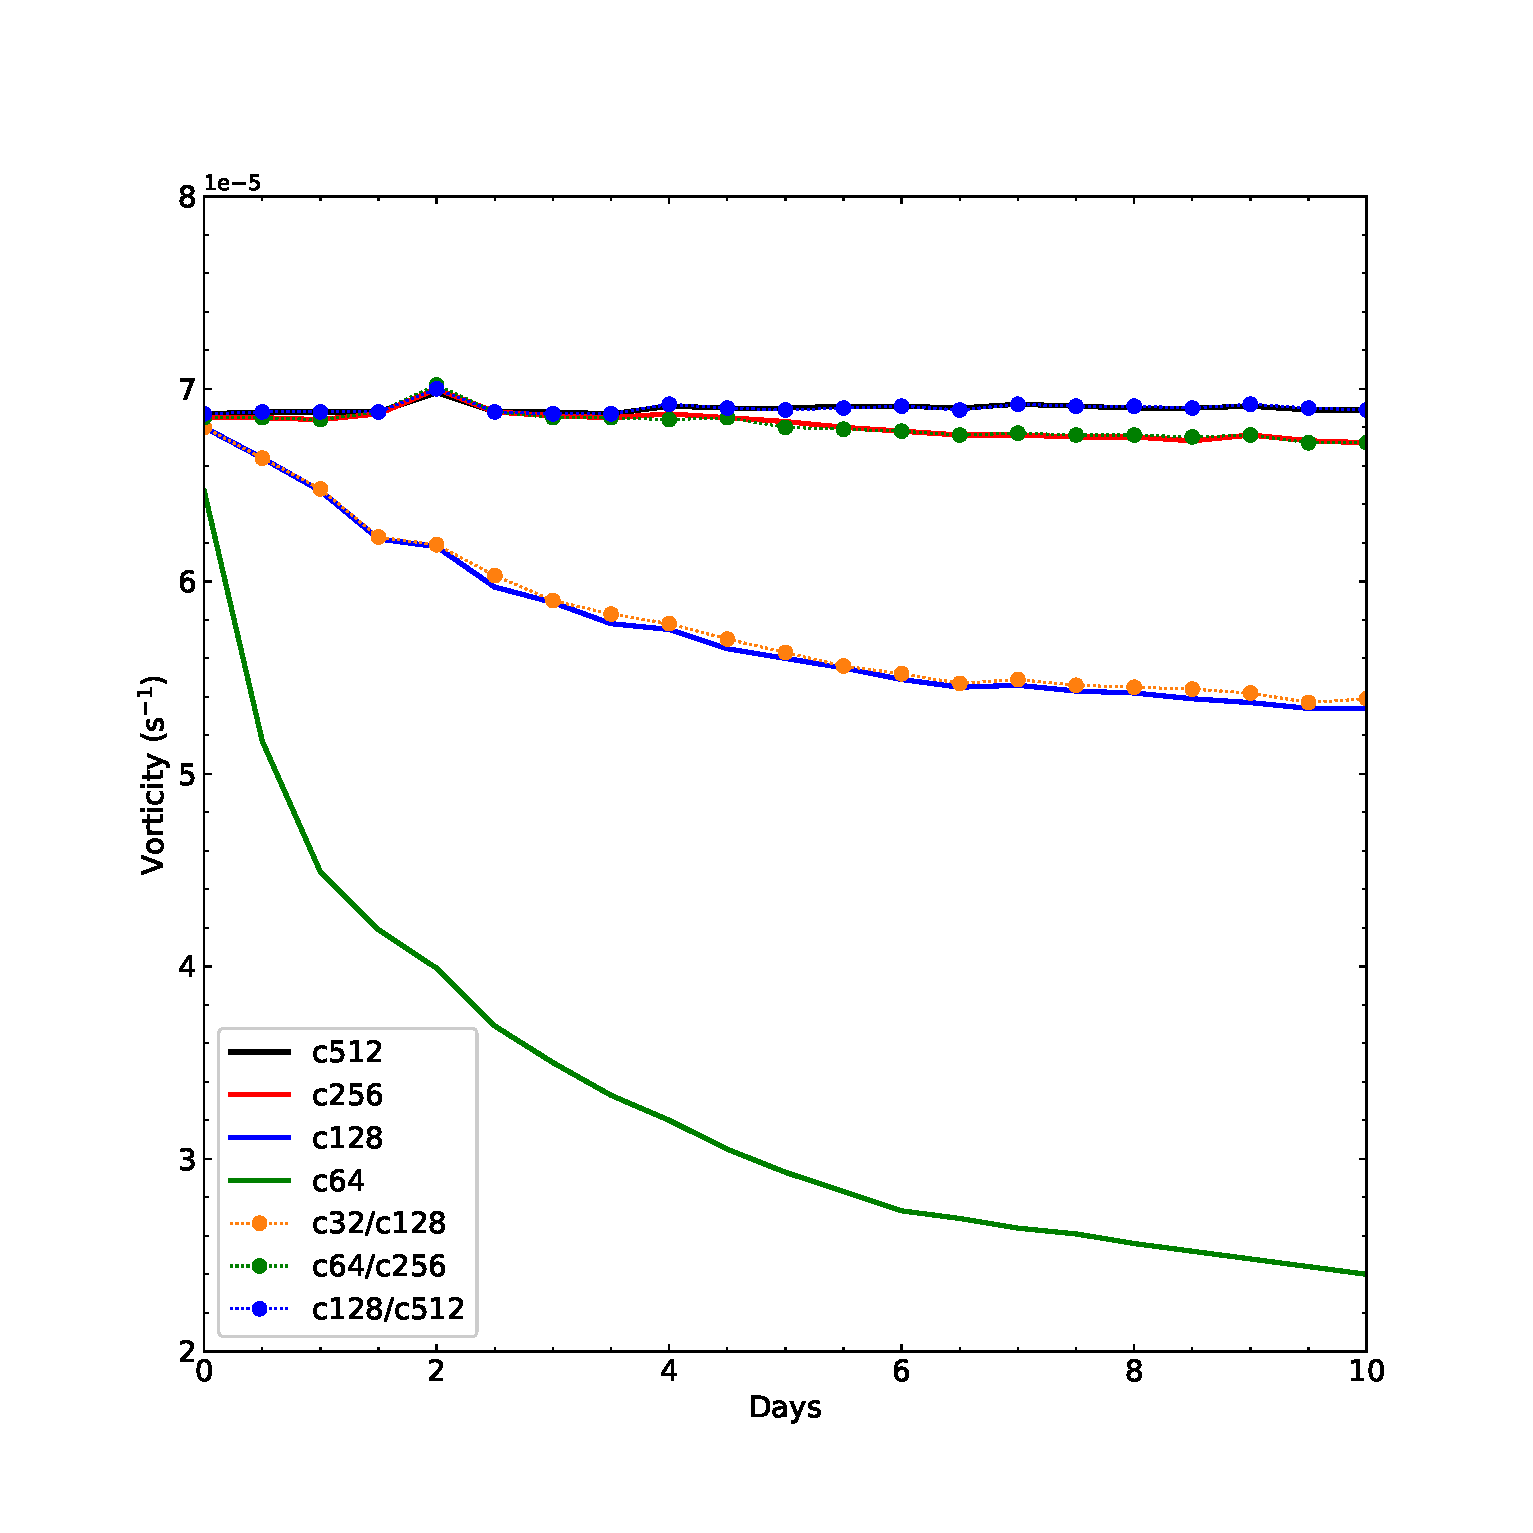
\includegraphics[width=\textwidth]{Chap3/modon_maxvort.eps}}
    \caption{10-day time evolution of the modons' maximum 
    vorticity for uniform and AMR runs.
}%
    \label{fig:modontevol}
\end{figure}

\subsection{Convergence tests}
We also use the modons test for some basic convergence tests
to assess the numerical methods. We compare
a series of uniform runs of varying resolutions and AMRs to
a uniform high-resolution reference solution. Since the modon test does not
have a known analytical solution, the c1024 uniform run in each scenario serves as
a reference solution. 
The normalized error measures for each run are
calculated via the traditional global error norms,
\begin{equation}
   \label{eq:l1_3d} L_1(h) = \frac{I\left[|h-h_\tau|\right]}{I\left[|h_\tau|\right]}
\end{equation}
\begin{equation}
   \label{eq:l2_3d} L_2(h) = \sqrt{\frac{I\left[(h-h_\tau)^2\right]}{I\left[h_\tau^2\right]}}
\end{equation}
\begin{equation}
   \label{eq:lmax_3d} L_\infty(h) = \frac{\max|h-h_\tau|}{\max|h_\tau|}
\end{equation}
where $h_\tau$ is the reference field and $I$ is a discrete approximation
to the global 3D integral given by
\begin{equation}
    \label{eq:globint_ed} I[x] = \sum_{\text{all cells } k} x_k V_k
\end{equation}
where $V_k$ denotes the volume of grid cell $k$.
With the finite-volume model, we expect fourth-order
convergence in the horizontal and second-order convergence in the vertical. However,
the time scheme is only second-order so the overall error convergence for any variable
tends towards second-order.

The 12-hour normalized errors as a function of grid resolution for density (left column) 
and vorticity (right column) are plotted in Fig. \ref{fig:largedterror}.
The runs depicted are uniform runs with resolution from c64 to c512
and three 1-level  x4 refinement AMR runs with c64, c128, and c256 base levels using the vorticity refinement criteria noted earlier.
These runs are implemented with the model's standard time step which fixes the CFL number at roughly $0.5$. With this,
the uniform c512 model has a time step of $\Delta t=20$ s, while the c64/c256 AMR run has a coarse fine step of $\Delta t =160$ s
and a sub-cycling time step of $\Delta t=40$ s for the c256 AMR level.  In the left column of Fig. \ref{fig:largedterror},
we observe second-order convergence in the $L_1$ (Fig. \ref{fig:largedterror}a) and $L_2$ (Fig. \ref{fig:largedterror}c) errors.
It is further reduced to first order for the $L_{max}$ in Fig. \ref{fig:largedterror}e.  Additionally, the AMR runs have roughly the same
errors as their base resolution uniform runs. No noticeable improvement is gained from the AMR; 
the vorticity tagging and refinement of only two localized areas is not 
expected to significantly improve global density errors.

We do observe improvements in the vorticity errors (Figs. \ref{fig:largedterror}b, d, and f) as a result of AMR. 
The c64/c256 AMR has higher errors than the uniform c256, but lower errors than the uniform c128 run 
in all three norms despite using roughly one-third the total number of grid cells in the c128 run.  The error improvement
is not as significant in the c256/c1024 AMR. This could be explained by the convergence of the solution at higher resolutions
resulting in diminishing returns for the benefits of AMR in improving global error \citep{lin2017colliding}.
Surprisingly, vorticity maintains a fourth-order convergence in the $L_1$ and $L_2$ error norm (Figs.  \ref{fig:largedterror}b and d)
and approximately third-order convergence in the $L_{max}$ norm (Fig.  \ref{fig:largedterror}f) even though it is not a prognostic variable, 
but derived from the momentum variables. By 24 hours, convergence does drop to second order for vorticity, 
and several days into simulation errors for all variables are first-order at best.

\begin{figure}
    \centerline{%
    \noindent
    \includegraphics[width=\textwidth,height=\textheight,keepaspectratio]{Chap3/long_run_normerrs-01.eps}}
    \caption{The 12 hour $L_1$ (a)-(b), $L_2$ (c)-(d), and $L_{max}$ (e)-(f) normalized errors for
    $\rho$ density (left column) and vorticity (right column) with
    respect to the uniform c1024 run for uniform and 1-level x4 refinement 
    AMR runs. The AMR runs are plotted with respect to their base resolutions.
    These runs used the standard time steps which results in
    a CFL number of around $0.5$ for all resolutions.
}%
    \label{fig:largedterror}
\end{figure}

To assess if the horizontal discretization is achieving fourth-order accuracy,
we can work to minimize the temporal error source, so that the error is dominated 
by the spatial discretization. To this end, we perform a second convergence study comparing
c32 through c512 resolution uniforms with a c1024 reference run.
The time step in these runs is set to have CFL number of approximately $1/160$ in contrast to the $0.5$ in the previous study. 
We also only perform the error analysis at $t=160$ s so the temporal error does not have time to build up.
Note these runs were run with 32 vertical levels (all previous runs had 16 levels) to create a smoother vertical transition of variables.
The $L_1$, $L_2$, and $L_{max}$ errors are plotted in Fig. \ref{fig:smalldterror} for density \ref{fig:smalldterror}a, 
momentum in the $\alpha$ direction \ref{fig:smalldterror}b, and vorticity \ref{fig:smalldterror}c.
The uniform grid resolutions c64 and higher display fourth-order convergence in all 
three error norms for both $\rho u_\alpha$ momentum in Fig. \ref{fig:smalldterror}b
and vorticity in Fig. \ref{fig:smalldterror}c. The convergence rates of the three error 
norms for the density variable diverge (Fig. \ref{fig:smalldterror}a).  The  
second-order convergence of the $L_1$ error reduces to first-order at higher resolutions. 
The $L_2$ error is approximately third-order convergent at resolutions c128 and below, but also 
reduces to first-order at the highest resolutions. In contrast, the $L_{max}$ density error 
exhibits fourth-order convergence except at the coarsest c32 and c64 resolutions.
The variations in density convergence could be attributed to the test case 
is not fully balanced. The models has to rapidly adjust to cyclostrophic balance. 
The error distortions could rise from the adjustment processes affecting the density 
field, though this question warrants further investigation to confirm it is not an artifact of an
issue with the model numerics.

\begin{figure}
    \centerline{%
    \noindent
    \includegraphics[height=.9\textheight]{Chap3/smalldt_normerrs-01.eps}}
    \caption{$L_1$, $L_2$, and $L_{max}$ normalized errors after $160$s 
    for (a) $\rho$ density, (b) $\rho u_\alpha$ momentum density, and (c) vorticity with
    respect to the uniform c1024 run. Small time steps are used which result in
     a CFL number of around $1/160$ for all resolutions.
}%
    \label{fig:smalldterror}
\end{figure}


\section{Idealized tropical cyclone}
\label{sec:tctest}

In the idealized TC test case by \cite{reed2012idealized}, a simple 
physics parameterization suit with the important driving mechanism of TCs
is added to the dycore. This causes
an initially weak vortex to rapidly intensify into a TC
and is a dynamic test case with real world applications.
We use the idealized TC to demonstrate AMR's effectiveness in tracking and resolving
the TC and asses how the physics forcing interacts with the AMR grid levels.
Its use is analogous to the 2D moist shallow water strengthening vortex test 
in Chapter \ref{chap:forcedsw}. A key focus area is the ability of the physics scheme
to handle changes in resolution, either at coarse-fine boundaries or when AMR is added
or removed. In addition, we are interested in assessing refinement criteria and AMR 
implementation timing effects on the evolution of the TC.

\subsection{Simple physics parameterization}
  The simple-physics parameterization suite of \cite{reed2012idealized}
  consists of three main mechanisms that drive tropical cyclone development.
  It implements a large-scale condensation mechanism that gets 
  triggered when the atmosphere becomes saturated. 
  The condensation scheme does not include a cloud stage, and it 
  instantaneously removes condensed moisture
  without any reevaporation at lower model levels. The 
  second component is a representation of the surface fluxes 
  that describe the interactions between the lower atmosphere and the ocean surface. 
  Specifically, it sets fluxes of horizontal momentum,
  sensible heat, and latent heat. The package assumes an aqua-planet surface with no topography
  and uniform sea surface temperatures. Finally, this scheme parameterizes boundary layer
  turbulence. For the Chombo AMR model, the physics time step is set to 16 minutes for all resolutions,
  comparable to the average physics time step
  used by models in \cite{reed2012idealized}. This time step is longer than 
  the dynamic time steps (40s to 6 mins, depending on resolution) used in this chapter.
  The frequency at which physics is called affects the evolution of the TC and
  is an area of further interest for AMR and the broad atmospheric modeling community.
  
\subsection{Idealized tropical cyclone}
  The initialization of the starting analytic vortex is
  described in detail by \cite{reed2011vortex}. The prescribed
  pressure, temperature, moisture, and velocity fields establish
  an initial vortex with initial maximum winds of $20$ m s$^{-1}$ located
  near the surface. The radius of maximum wind of roughly 250 km. The
  vortex is embedded in a background designed to
  mimic favorable tropical conditions.
  The background surface pressure is set to $p_0 = 1015$ hPa
  and the background wind at all vertical levels is zero.
  The model top height is set to 30 km and a stretched mapping is implemented
  in the height-based vertical coordinates.
  The mapping smoothly
  concentrates vertical levels closer to the surface to improve the resolution
  of the tropical cyclone and the physics processes that force it.

\begin{figure}
    \centerline{%
    \noindent
    \includegraphics[width=\textwidth]{Chap3/c256_intime-01.eps}}
    \caption{Snapshots of the tropical cyclone at day 3 (left), day 5 (middle), and day 10 (right)
    for the uniform c256 model run. (a)-(c) Surface pressure. (d)-(f) Wind speed at
    a height of 250 m. (g)-(i) Longitude-height cross-section of the wind speed through the center
    latitude of the vortex.
}%
    \label{fig:c256intime}
\end{figure}

   Figure \ref{fig:c256intime} depicts the evolution of the TC in 
   a c256 ($0.35^\circ$) uniform resolution run as it beta-drifts
   northwestward due to the Coriolis force over a period of ten days. The leftmost column shows 
   the surface pressure (Fig. \ref{fig:c256intime}a),
   the wind speed at 250m (Fig. \ref{fig:c256intime}d), and the vertical cross-section 
   of the wind speed (Fig. \ref{fig:c256intime}g). The middle column (Figs. \ref{fig:c256intime}b, e, and h)
   are the same plots for day 5, and the rightmost column (Figs. \ref{fig:c256intime}c, f, and i)
   depicts day 10.
   
   The c256 resolution is the highest resolution used for these simulations. As resolution
   increases, certain wave modes in the vertical components grow stronger and become unstable between
   the first and second day of the simulation. This time corresponds to the start of significant TC strengthening 
   which drives a rapid increase in vertical velocity at the TC's center. 
   The unstable modes add to this growth, eventually triggering CFL violations that stop the simulation.
   This instability can be mitigated by further decreasing the time step at higher resolutions. 
   However, such methods are not sustainable, as resolutions c512 or beyond require 
   time steps that are too small, making the simulation prohibitively costly to run. 
   Determining the causes of these unstable modes and possible solutions is an
   ongoing effort. For this reason, the highest resolution implemented for the TC test in uniform 
   or AMR mode is c256.


\subsection{AMR with the idealized TC}
In addition, to the uniform c256 run, we also ran uniform c64 and c128 runs.
We implemented four different refinement criteria for use in the AMR runs.
\begin{itemize}
    \item
        Tag 1 is a surface pressure threshold tag based on the
        absolute difference from the initial surface pressure $p_0=1015$ hPa. Refinement 
        is triggered where $|p_s - p_0| > 4$ hPa.
    \item
        Tag 2 is a relative vorticity threshold that refines where
        $|\zeta| >  2 \times 10^{-5} \mathrm{s}^{-1}$.
     \item
        Tag 3 is a relative vorticity threshold that refines where
        $|\zeta| > 1 \times 10^{-5} \mathrm{s}^{-1}$.
     \item
        Tag 4 is a surface pressure tag that refines where
        $|p_s - p_0| > 9$ hPa.
\end{itemize}
An overview of all simulations performed for this section, including the run resolutions and 
AMR refinement criteria used, is presented in Table \ref{tb:tcruns}.

\begin{table}[h]
  \caption{Brief description of all uniform and AMR runs performed for Sec. \ref{sec:tctest}.
  For each run the model resolutions, the refinement criteria (Tags 1 through 4), and the tagging variable are presented.
  Some of the AMR simulations have prescribed delays that prevent refinement from occurring until
  after a set time. That delay, in hours, is shown in the right most column. 
  The model resolutions (left most column) are presented in cubed-sphere coordinates ($cN$) with N
  being the number of cells along each panel edge.
  For the AMR runs, the resolutions for the multiple levels are given in the form c32/c128/c512, where the
  left most resolution is the base level's resolution and the subsequent 
  resolutions are for each level of AMR implemented.
  }
  \label{tb:tcruns}
  \begin{center}
 %    \resizebox{\textwidth}{!}{
  \begin{tabular}{lccc}
     \hline
     Run Resolution & AMR Criteria & Tagging Variable & Delay (hrs) \\
     \hline
     \hline
     c16/c64/c256 	& Tag 3	& Vorticity			& 0 \\
     c32/c128		& Tag 1	& Surface Pressure	& 0 \\
     c32/c128		& Tag 2	& Vorticity			& 0 \\
     c64			& - 		& - 				& - \\
     c64/c256		& Tag 1	& Surface Pressure	& 0 \\
     c64/c256		& Tag 2	& Vorticity			& 0 \\
     c64/c256		& Tag 3	& Vorticity			& 0 \\
     c64/c256		& Tag 4	& Surface Pressure	& 0 \\
     c64/c256		& Tag 1	& Surface Pressure	& 48 \\
     c64/c256		& Tag 3	& Vorticity			& 24 \\
     c64/c256		& Tag 3	& Vorticity			& 48 \\
     c128			& -		& -				& - \\
     c256			& -		& -				& - \\
     \hline
  \end{tabular}
%     }
  \end{center}
\end{table}

\begin{figure}
    \centerline{%
    \noindent
    \includegraphics[height=.9\textheight]{Chap3/TC_amr_plots-01.eps}}
    \caption{Time evolution of the (a) minimum surface pressure and (b) maximum
    wind speed at 250m for three uniform runs and six AMR runs
    using various refinement criteria.
}%
    \label{fig:timeevolplots}
\end{figure}

Figure \ref{fig:timeevolplots} depicts the time evolution of the minimum surface
 pressure (Fig. \ref{fig:timeevolplots}a) and maximum wind speed at a height 
 of 250 m (Fig. \ref{fig:timeevolplots}b) for the three uniform runs and six AMR 
 runs using the first three tagging criteria. We observe that
the c256 run has a minimum surface pressure of around 920 hPa by day 10. This is
comparable to the strongest TC produced in \cite{reed2012idealized} using the 
simple physics scheme. Wind speeds in \cite{reed2012idealized} were calculated 
at 100 m, making direct comparisons difficult. In the uniform c64 run, the TC slowly
weakens initially. After day 3 it starts to strengthen but at a much slower rate 
than the higher resolution runs. By day 10, its maximum wind speed is less than half the 
c256 uniform run.
In \ref{fig:timeevolplots}, the four AMR runs that have a c256 level of refinement track the 
evolution of the uniform c256 TC closely. The two c32/c128 AMR runs also follow the uniform 
c128 run's progression but not as closely. Both the Tag 1 and Tag 2  c32 base AMR runs diverge 
markedly at several points during the ten days.
In all six AMR runs, the refinement threshold is met initially so that the TC is resolved by 
the highest level of AMR for the entire simulation.

\begin{figure}
    \centerline{%
    \noindent
    \includegraphics[width=\textwidth,height=\textheight,keepaspectratio]{Chap3/windspeed_amr-01.eps}}
    \caption{
    Day 10 snapshots of the horizontal wind speed at 250m for three uniform runs,
    (a) c64, (d) c128, and (g) c256, and the six AMR runs also depicted in 
    Fig. \ref{fig:timeevolplots}.
}%
    \label{fig:hwindsamr}
\end{figure}

\begin{figure}
    \centerline{%
    \noindent
    \includegraphics[width=\textwidth,height=\textheight,keepaspectratio]{Chap3/panel_vertwind_day10-01.eps}}
    \caption{
    Day 10 snapshots of the longitude-height cross-section
     of the wind speed through the center
    latitude of the vortex, for the same
    uniform and AMR runs as in Fig. \ref{fig:hwindsamr}.
}%
    \label{fig:vertwindsamr}
\end{figure}

The wind fields at a height of 250 m for all nine runs are shown in Fig. \ref{fig:hwindsamr}. 
The vertical cross-section of the wind fields centered around the
strongest vortex are plotted in Fig. \ref{fig:vertwindsamr}. From the uniform 
runs we observe increasing strength with increasing resolution
as well increasing compactness, a recognized sensitivity of simple physics 
\citep{reed2012idealized}. The TC strength and structure in the AMR runs compare well to
the corresponding uniform runs.  The main exception to this similarity is
the secondary vortex which spins up at the main TC's origin point. 
This TC is another resolution-sensitive feature, that is only produced in 
some models in \cite{reed2012idealized}.
In our simulation all three uniform runs have the secondary vortex developing, 
though it is only clearly defined in the c256 run. However, only half of the 
AMR runs develop this secondary vortex.
It develops in both Tag 3 AMR runs which have the broadest refinement, 
though it is fairly weak in Fig. \ref{fig:hwindsamr}h and much stronger than 
the c256 uniform run in the c64/c256 AMR run (Fig. \ref{fig:hwindsamr}i). 
Neither Tag 2 AMR runs develop the secondary vortex, and only the lower resolution 
c32/c128 surface pressure based AMR run (Fig. \ref{fig:hwindsamr}b) develops 
it. In Fig. \ref{fig:hwindsamr}b. the main TC is also significantly 
weaker than either the c128 uniform run (Fig. \ref{fig:hwindsamr}d) or the other 
c32/c128 AMR run (Fig. \ref{fig:hwindsamr}e) This main vortex is weakened by the
secondary vortex interfering with the main 
vortex's source of heat and moisture. This also explains the weakened eastern side of the
c64/c256 Tag 3's main TC, seen in Fig. \ref{fig:vertwindsamr}i. 
\cite{reed2012idealized} observed that small perturbations in the initial vortex structure 
led to noticeable spread in the evolution of the TC. So it is not
unexpected that differences in AMR grid locations can affect the evolution of the secondary vortex.
The tertiary vortex that appears in
the c16/c64/c256 AMR run (Fig. \ref{fig:hwindsamr}h) on the polar panel edge north of the main vortex
is a numerical artifact from the same AMR/panel edge issue observed in the modon tests.

\begin{figure}
    \centerline{%
    \noindent
    \includegraphics[height=.9\textheight]{Chap3/TC_delayed_plots-01.eps}}
    \caption{Time evolution of (a) minimum surface pressure and (b) maximum
    wind speed at 250m for three uniform runs and four AMR runs
    that do not have initial refinement over the vortex.
}%
    \label{fig:delayedplots}
\end{figure}

Initiating refinement at
the start of the simulation minimizes the growth of 
early coarse grid errors that carry over to the finer grids. 
In more realistic scenarios, a
distinct initial condition to tag on may not always be present. 
We are therefore interested in studying how the idealized TC and the simple physics mechanisms will
adjust to the addition of resolution when AMR is triggered a few 
days into the simulation rather than initially. 
The tag 4 criterion has a refinement threshold that is higher than the initial 
maximum surface pressure spread, so refinement is delayed
until the TC undergoes some strengthening on the coarse grid. Due 
to the high threshold though, the newly triggered AMR grid fails to sufficiently 
cover the whole TC for several additional days. To explore more refinement 
options, we implement an artificial delay to refinement. For the Tag 1 
and Tag 3 criteria, we manually shut off tagging in the model for either 24 
or 48 hours.  After that cut off, a broad area of refinement is applied over the TC.
Figure \ref{fig:delayedplots} shows the time evolution of the minimum surface
pressure (Fig. \ref{fig:timeevolplots}a) and maximum wind speed at a height 
of 250 m (Fig. \ref{fig:timeevolplots}b) for the four AMR runs.  The uniform 
runs are again plotted for comparison purposes. Figures \ref{fig:delayhwind} 
and \ref{fig:delayvertwind} depict the horizontal and vertical cross-sections of
the winds of the three AMR runs, respectively, with the uniform c256 run 
serving as a reference. 
The c64/c256 Tag 3 AMR run with a 48-hour delay was stopped at day 7 by 
the vertical velocity instability discussed at the beginning of this section, so
it is not pictured in these plots.

\begin{figure}
    \centerline{%
    \noindent
    \includegraphics[width=\textwidth,height=\textheight,keepaspectratio]{Chap3/day10_wind_amrdelayed-01.eps}}
    \caption{
    Day 10 snapshots of the horizontal wind speed at 250m for the three AMR runs
    that do not have initial refinement over the vortex. (a) Uniform c256, for reference.
    (b) c64/c256 using a tagging criterion of $|\Delta p| > 9$hPa. (c) c64/c256
    using Tag 3 with a 24-hour delay. (d) c64/c256 using Tag 1 with a 48-hour delay.
}%
    \label{fig:delayhwind}
\end{figure}

\begin{figure}
    \centerline{%
    \noindent
    \includegraphics[width=\textwidth,height=\textheight,keepaspectratio]{Chap3/day10_vertwind_amrdelayed-01.eps}}
    \caption{
    Day 10 snapshots of the jongitude-height cross-section
     of the wind speed through the center
    latitude of the vortex, for the same
    uniform and AMR runs as in Fig. \ref{fig:delayhwind}.
}%
    \label{fig:delayvertwind}
\end{figure}
 
The c64/c256 Tag 4 AMR run triggers refinement after three days. 
Figure \ref{fig:delayedplots} shows the drop in surface pressure and sharp 
jump in wind speed, however the AMR does not sufficiently cover the 
vortex resulting in the TC's strength fluctuating around the uniform c64 TC's level
despite refinement. In contrast, by day 10 the TC in the c64/c256 Tag 1 AMR 
run with a 48-hour delay has strengthened to c256 TC comparable wind speeds and surface pressure levels. Its
AMR is triggered after two and a half days but refines a broader area, capturing the whole TC. 
Once the refinement is triggered, the TC strengthens consistently until day 10, 
but the increase is not as rapid as the other delayed AMR runs.
This is also true in comparison to  the
initial strengthening of the c128 and c256 uniform runs. 
The TCs in the two delayed Tag 3 AMR runs follow similar trajectories.
After the delay, refinement is immediately triggered over the whole TC and the surrounding area. The 
TC undergoes an abrupt transition that temporarily distorts the vortex structure for approximately 24 hours and causes it to rapidly strengthen.
The evolution of the c64/c256 Tag 3 AMR run with the 24-hours delay mimics 
the rapid strengthening of the uniform c256 TC, merely a day behind.  By day 6, 
the minimum surface pressure and wind speed in the Tag 3 AMR 
and the c256 uniform runs are approximately the same.
At day 10, Figs. \ref{fig:delayhwind} and \ref{fig:delayvertwind} 
shows that both the Tag 1 and Tag 3 delayed
runs have TCs comparable to the uniform c256 TC. The c64/256 Tag 3 delayed run
even captures the development of the 
secondary vortex (Fig. \ref{fig:timeevolplots}c).
The processes in the evolution of the high resolution TC can still be 
triggered in AMR runs that do not have high levels of refinement initially.
These AMR runs demonstrate a time window during which the TC can undergo rapid strengthening
and evolve into a vortex comparable to the TC from the uniform high resolution run.

\section{Conclusions}
\label{sec:conclusion3}

In this chapter, we used the non-hydrostatic finite-volume Chombo AMR dycore
and demonstrated its AMR characteristics for idealized 3D atmospheric flows on the sphere.
 We implemented two test cases: the colliding modons
test, in the dry dycore and the idealized TC test with an added simple moist physics parameterization package.
In the modon test, AMR functioned as expected. It was able to tag, refine, and follow the modons
and it effectively reduced the global vorticity errors.
The error convergence properties met our expectations given 
the implemented numerical schemes and the current status of the model.
However, a few notable results trigger the need for further investigations.
Several stability problems were observed in both test cases that need to
be better understood and corrected.

In the idealized TC test, the AMR runs were able to effectively reproduce results from uniform high resolution runs.
The physics scheme was able to function effectively over multiple levels of refinement. No noise
or instabilities were observed at coarse-fine boundaries, though some
 numerical artifacts were observed on polar panel edges. 
Several aspects of the TC's evolution were
sensitive to the tagging criteria and AMR coverage such as the generation of the secondary vortex.
Having  AMR levels applied initially is the most effective way of improving results.
However, the delayed AMR tests demonstrated that the TC can still 
undergo the same strengthening processes as high resolution runs once refinement is triggered.
There is a narrow window of flexibility, in which the triggering of AMR allows the TC in the AMR 
run to catch up to the results in the high resolution uniform run.
The most promising refinement technique is a combination of some initial 
refinement and AMR. The initial refinement limits error growth at the 
base resolution and ensures that the model can resolve the feature of interest. 
Additional AMR level then enable the feature to then be fully resolved.



